
% \section{Safe Alignment via Risk and Dominance}

We now present our safe alignment formulation -- \emph{Risk-sensitive Alignment via Dominance  (RAD)}. Standard Safe RLHF constrains the \emph{expected} cost, which controls only a single moment of the cost distribution.
% RAD instead enforces a \emph{distributional} safety constraint using first-order stochastic dominance (FSD), implemented via the asymmetric FSD cost $\mathcal{L}_{\mathrm{FSD}}$ (Eq.~\eqref{eq:fsd_loss}).
RAD instead enforces a \emph{distributional} safety constraint using first-order stochastic dominance (FSD). We first introduce FSD as a principled way to ensure the learned policy's cost distribution is
stochastically smaller than a reference,
% \yc{stochastically smaller again}
implemented via the asymmetric FSD surrogate $\mathcal{L}_{\mathrm{FSD}}$ (Eq.~\eqref{eq:fsd_loss}). We then show that reweighting quantiles of this surrogate recovers
Spectral Risk Measures (SRMs), yielding a unified framework in which the choice of weighting function $w(q)$ controls the risk profile of the learned policy.
Recall that our reward model is denoted by $r_{\phi}(x,y)$ and our cost model is denoted by $c_{\psi}(x,y)$ for input $x$ and ouptut $y$ and for learned parameters $\phi$ and $\psi$. For a policy $\pi$, let $C_\pi := c_\psi(x,y)$ denote the random variable of costs induced by sampling
$x\sim\mathcal{D}_x$ and $y\sim\pi(\cdot\mid x)$. Thus, we solve:
\begin{align}
  \max_\theta \quad & \mathbb{E}_{x\sim D_x,\,y\sim\pi_\theta(\cdot\mid x)}\!\Big[r_\phi(x,y)\Big]
  - \beta\,D_{\mathrm{KL}}\!\big(\pi_\theta(\cdot\mid x)\,\|\,\pi_{\mathrm{ref}}(\cdot\mid x)\big), \label{eq:sard_primal_obj}\\
  \text{s.t.}\quad & \mathcal{L}_{\mathrm{FSD}}\!\big(C_{\pi_\theta},\,C_{\pi_{\mathrm{ref}}}\big)\;\ge\;\kappa. \label{eq:sard_primal_constr}
\end{align}
Constraint~\eqref{eq:sard_primal_constr} encourages \emph{uniform} improvement across quantiles: since
$\mathcal{L}_{\mathrm{FSD}}(C_{\pi_\theta},\,C_{\pi_{\mathrm{ref}}})=\int_0^1 (Q_{C_{\pi_{\mathrm{ref}}}}(q)-Q_{C_{\pi_\theta}}(q))_+\,dq$,
larger values of $\mathcal{L}_{\mathrm{FSD}}\!\big(C_{\pi_\theta},C_{\pi_{\mathrm{ref}}}\big)$ correspond to larger positive gaps $Q_{C_{\pi_{\mathrm{ref}}}}(q)-Q_{C_{\pi_\theta}}(q)$ over $q\in[0,1]$.
Equivalently, it encourages $C_{\pi_{\mathrm{ref}}}\succeq_{\mathrm{FSD}} C_{\pi_\theta}$, i.e., the learned policy has stochastically smaller costs. %\yc{stochasticall smaller again}.
% pushes the learned-policy cost quantiles downward relative to the reference across the distribution, not only in expectation.

To optimize our objective, we first absorb the KL term into the reward by defining the KL-regularized reward
$\tilde r(x,y)= r_\phi(x,y)-\beta\log \frac{\pi_\theta(y\mid x)}{\pi_{\mathrm{ref}}(y\mid x)}$ as done in \cite{dai2023safe},
and then use Dual Ascent \citep{gallier2019fundamentals} to optimize the Lagrangian relaxation of \eqref{eq:sard_primal_obj}--\eqref{eq:sard_primal_constr}:
\begin{equation}
  \max_\theta\min_{\lambda\ge 0}\;\underbrace{
    \mathbb{E}_{x\sim D_x,\,y\sim\pi_\theta(\cdot\mid x)}\!\Big[\tilde r(x,y)\Big]
  +\lambda\Big(\mathcal{L}_{\mathrm{FSD}}\!\big(C_{\pi_\theta},C_{\pi_{\mathrm{ref}}}\big)-\kappa\Big)}_{L(\theta,\lambda)}. \label{eq:sard_dual}
\end{equation}

\paragraph{Non-parametric (quantile-particle) representation of policy-induced cost distributions.}
\label{subsec:nonparam}
We now describe how we represent the cost distributions for our policies.
For a policy $\pi$, rather than assuming a parametric family for the cost distribution $C_\pi$, we use a non-parametric empirical approximation
via particles in the \emph{quantile space}. Fix quantile levels $\alpha_1,\dots,\alpha_N\in(0,1)$ and define the corresponding
cost-quantile particles:
\begin{equation}
  q_i(\pi) := Q_{C_\pi}(\alpha_i),\qquad i=1,\dots,N,
  \label{eq:quantile_particles}
\end{equation}
which we assume are ordered so that $q_1(\pi)\le \cdots \le q_N(\pi)$.
We approximate the cost distribution by the empirical measure:
\begin{equation}
  \hat\mu_\pi := \frac{1}{N}\sum_{i=1}^N \delta_{q_i(\pi)}.
  \label{eq:empirical_measure}
\end{equation}
In practice, $\hat\mu_\pi$ is obtained by sampling generations from $\pi$, evaluating their costs via $c_\psi$,
and computing empirical quantiles from the resulting samples; these quantiles serve as the particles defining the discrete
representation. Let $\hat{\mu}_{\pi_{\theta}}$ and $\hat{\mu}_{\pi_{\mathrm{ref}}}$ be the empirical measures for the cost distrivutions corresponding to policies $\pi_{\theta}$ and $\pi_{\mathrm{ref}}$ respctively. Then, the FSD objective is approximated as $\mathcal{L}_{\mathrm{FSD}}\!\big(C_{\pi_\theta},\,C_{\pi_{\mathrm{ref}}}\big) \approx \mathcal{L}_{\mathrm{FSD}}\!\big(\hat{\mu}_{\pi_{\theta}},\,\hat{\mu}_{\pi_{\mathrm{ref}}}\big)$. %\yc{commented out the equation below. Lmk if this is needed}\aj{works}
% The FSD objective between two such policy-induced cost distributions $C_{\pi_\theta}$ and $C_{\pi_{\mathrm{ref}}}$ is given by:
% \begin{equation}
%   \mathcal{L}_{\mathrm{FSD}}\!\big(C_{\pi_\theta},\,C_{\pi_{\mathrm{ref}}}\big) \approx \mathcal{L}_{\mathrm{FSD}}\!\big(\hat{\mu}_{\pi_{\theta}},\,\hat{\mu}_{\pi_{\mathrm{ref}}}\big)
%   \;=\;
%   \frac{1}{N}\sum_{i=1}^N \big(q_i(\pi_{\mathrm{ref}})-q_i(\pi_\theta)\big)_+.
%   \label{eq:fsd_sum_approx}
% \end{equation}
\paragraph{Computing the RAD policy gradients.}
% \yc{removed the part about non-differentiability, as subgradients do work. Can be a reviewer headache. Just mention the challenge is the gradient of the FSD term wrt theta}
% The main technical challenge for computing the gradients of the RAD policy is differentiating the FSD term in~\eqref{eq:fsd_sum_approx} with respect to the quantiles efficiently. The FSD objective is not smooth with respect to particle positions. It is also non-differentiable and small perturbations in particle locations can induce discontinuous changes in the gradient.
The main technical challenge for computing the gradients of the RAD policy is differentiating the FSD term with respect to the policy parameters $\theta$.
To compute the gradients of the FSD objective effectively, first note that it can be interpreted as an optimal transport problem between the two cost distributions as described in~\eqref{eq:otl}. On adding entropic regularizion, the resulting optimization problem in~\eqref{eq:ot-unreg} is strictly convex and differentiable. Moreover, the entropic regularized optimal problem has smooth gradients and the unique minimizer of the objective can be computed efficiently using Sinkhorn iterations. Hence, we replace the FSD objective with the entropic regularzied FSD objective $\mathcal{L}^{\chi}_{\mathrm{FSD}}$ where $\chi$ is the regularization parameter (as in~\eqref{eq:ot-unreg}) \yc{$\beta$ already used in KL regularized rewards. Change this to $\chi$} \aj{We are also using the superscript for the weighted version of $\mathcal{L}$}. We next state the resulting policy-gradient estimator; the full derivation and implementation details are deferred to Supplementary Material ~\ref{app:sard_pg_derivation}.

\begin{theorem}[RAD policy-gradient estimator]\label{thm:sard_pg}
  Fix $\lambda\ge 0$ and define the dual objective $L(\theta,\lambda)$ by \eqref{eq:sard_dual}.
  Let $\alpha_1,\dots,\alpha_N\in(0,1)$ be fixed quantile levels and let
  $q_i(\pi_\theta):=Q_{C_{\pi_\theta}}(\alpha_i)$ denote the corresponding cost-quantile values. Using the empirical quantile-particle approximation from \Cref{eq:empirical_measure},
  the gradient $\nabla_\theta L(\theta,\lambda)$ admits the REINFORCE-form estimator
  \begin{equation}
    \nabla_\theta L(\theta,\lambda)
    =
    \mathbb{E}_{x\sim D_x,\,y\sim\pi_\theta(\cdot\mid x)}
    \Bigg[
      \Bigg(\tilde r(x,y)+\lambda\sum_{i=1}^N
        \Big(-\frac{\partial \mathcal{L}^{\chi}_{\mathrm{FSD}}}{\partial q_i(\pi_\theta)}\Big)\,
        \mathbf{1}\!\big(c_\psi(x,y)\le q_i(\pi_\theta)\big)
      \Bigg)
      \nabla_\theta\log\pi_\theta(y\mid x)
    \Bigg]. \label{eq:sard_pg}
  \end{equation}
  Moreover, for the weighted dominance objective $\mathcal{L}^{w}_{\mathrm{FSD}}$ (see \Cref{eq:weighted-fsd-loss-dfn}),
  the same estimator holds with an additional factor $w(\alpha_i)$ multiplying the $i$th summand. %\aj{Weighted FSD loss hasn't been introduced yet}
\end{theorem}
% \aj{Is the following line correct? REINFORCE \citep{williams1992simple} with RLOO \citep{Kool2019Buy4R} and Dual Ascent \citep{gallier2019fundamentals} were mentioned in the previous draft.}
We optimize \eqref{eq:sard_dual} by alternating (i) ascent in $\theta$ using \eqref{eq:sard_pg} with REINFORCE \citep{williams1992simple} and variance-reduction scheme (RLOO) \citep{Kool2019Buy4R}, and (ii) Dual Ascent \citep{gallier2019fundamentals} in $\lambda$ to enforce the constraint.

% \aj{------------------------------}

% We now propose our approach: \underline{\textbf{Safe Alignment via Risk and Dominance (RAD)}}. Instead of enforcing a constraint on the expected costs of the model generations, which ignores tail risks, we propose a stochastic dominance constraint that ensures that the cost distribution of reference model generations dominates the cost distribution of the model generations. Stochastic Dominance offers a principled framework for capturing distributional uncertainity, unlike expected value constraints that only represent a snapshot/statistic of the cost ditribution. But, imposing a raw First-Order Stochastic Dominance (FSD) constraint makes the optimization harder, becuse FSD only imposes a partal ordering over distributions. Hence, we relax the FSD constraint to the metric $\mathcal{L}_{\mathrm{FSD}}$, proposed in Equation ~\ref{eq:fsd-loss}. The RAD objective is provided below:

% \begin{align}
%   \max_{\theta} \text{\space} &\mathbb{E}_{x \sim \mathcal D_x, y \sim \pi_{\theta}(\cdot \vert x)}[r_{\phi}(x,y)] - \beta \mathbb{D}_\mathrm{KL}\big(\pi_{\theta}(.\vert x) \vert\vert \pi_\mathrm{ref}(. \vert x)\big) \label{eq: sard-objective}\\
%   %
%   \text{s.t.} \quad & \mathcal{L}_{\mathrm{FSD}}(c_{\psi}(\pi_{\theta}), c_{\psi}(\pi_{\mathrm{ref}})) \geq \kappa. \label{eq: sard-constraint}
% \end{align}

% In the Constraint in Equation ~\ref{eq: sard-constraint}, $c_{\psi}(\pi_{\theta})$ and $c_{\psi}(\pi_{\mathrm{ref}})$ denote the random variables representing the distribution of costs of the model's and the reference model's generations respectively, for prompts $x \sim \mathcal{D}_{x}$. The constraint enforces that the cost distribution of the reference policy first-order stochastically dominates that of the learned policy by at least a value of $\kappa$. Operationally, this encourages the optimizer to identify a policy whose quantile costs are uniformly lower than those of the reference policy across quantile levels, with a gap of at least $\kappa$. In other words, improvements are promoted not merely in expectation but throughout the distribution, including high-cost regions. Notably, the present formulation weights all quantile levels equally, assigning uniform importance across the entire cost spectrum.

% Henceforth, we subsume the KL penalty into the rewards, using the KL regularized reward $\Tilde{r}(x,y) = r_{\phi}(x,y) - \beta \log \frac{\pi_{\theta}(y \vert x)}{\pi_{\mathrm{ref}}(y \vert x)}$ as the objective we want to maximize, subject to a FSD constraint that ensures the cost distribution of the reference policy's generations dominates that of our policy's generations by a value of atleast $\kappa$.

% To solve (\ref{eq: sard-objective}), we use lagrangian relaxation \citep{boyd2004convex} and covert the convert the constrained primal problem into a dual problem, with a lagrangian multiplier $\lambda \geq 0$, that we optimize using Dual Ascent \citep{gallier2019fundamentals}.

% \begin{align}\label{eq:RAD-dual}
%   \max_{\theta} \min_{\lambda \geq 0} \text{\space} &\mathbb{E}_{x \sim \mathcal D_x, y \sim \pi_{\theta}(.\vert x)}\Big[\Tilde{r}(x,y)\Big] + \lambda \Big(\mathcal{L}_{\mathrm{FSD}}(c_{\psi}(\pi_{\theta}), c_{\psi}(\pi_{\mathrm{ref}})) - \kappa\Big).
% \end{align}

% To optimize the objective in Equation~\ref{eq:RAD-dual}, we require its gradient with respect to $\theta$. While the gradient of the reward term can be computed using standard policy gradient techniques, differentiating the FSD loss term is considerably more involved. In particular, evaluating this term entails either computing an intractable integral over quantile levels or solving an optimal transport problem, even for a single forward pass. We therefore derive an estimator for the policy gradient of the Dual RAD objective next.

% \aj{Add the policy gradient estimate as a thm here, and move the rest of the section to the appendix. Can give a brief sketch in 2-3 lines.}

\subsection{Universality of Weighted FSD for Controlling Spectral Risk Measures}\label{subsec:srm}

% \textcolor{red}{Scott: UNIFICATION IS NOT EMPHASIZED HERE AT ALL. MAYBE THIS IS NOT UNIFICATION, since FSD IS NOT AN SRM. UNIVERSALITY OF FSD FOR REASONING ABT SPECTRAL RISK MEASURES (something like this)}

We now describe how we can change the FSD objective to represesnt various spectral risk measures. The FSD objective in Equation~\ref{eq:fsd_loss} weights all quantiles equally.
However, in many applications, tail performance is of primary concern, and it may be desirable to emphasize higher quantiles more heavily than lower ones.
To accommodate this, we introduce a quantile-weighted FSD objective with a nonnegative weighting function $w(q)$:
\begin{equation}
  \mathcal{L}_{\mathrm{FSD}}^{w}(X,Y)
  =
  \int_{0}^{1} w(q) \big(Q_{Y}(q) - Q_{X}(q)\big)_{+} dq,
  \label{eq:weighted-fsd-loss-dfn}
\end{equation}
where $w(q) \ge 0$ for all $q \in [0,1]$ and $\int_0^1 w(q) dq = 1$. While $\mathcal{L}_{\mathrm{FSD}}^{w}(X,Y)$ is not itself a spectral risk measure (SRM), it admits a direct structural relationship to the entire class of SRMs.
Recall that a spectral risk measure associated with weight function $w$ is defined as
\(
  \rho_w(Z) := \int_0^1 Q_Z(q)\, w(q)\, dq.
\)
Note that we have the following relationship:
\begin{equation}
  \int_{0}^{1} w(q) \big(Q_{Y}(q) - Q_{X}(q)\big) dq
  =
  \rho_w(Y) - \rho_w(X).
\end{equation}

Thus, weighted quantile differences correspond exactly to differences in spectral risk measures.
The following proposition formally states that the weighted FSD violations provide a decomposition of spectral risk differences.

\begin{proposition}
  Let $w : (0,1) \to \mathbb{R}_{+}$ be any nonnegative weight function with $\int_0^1 w(q) dq = 1$, and define
  \(
    \rho_w(Z) := \int_0^1 Q_Z(q)\, w(q)\, dq .
  \)
  For two random variables $X$ and $Y$, define
  {\small
    \[
      \mathcal{L}_{\mathrm{FSD}}^{w}(X,Y)
      :=
      \int_0^1 \big(Q_Y(q) - Q_X(q)\big)_+\, w(q)\, dq,
      \quad
      \mathcal{L}_{\mathrm{FSD}}^{w}(Y,X)
      :=
      \int_0^1 \big(Q_X(q) - Q_Y(q)\big)_+\, w(q)\, dq.
    \]
  }
  Then,
  {\small
    \[
      \rho_w(Y) - \rho_w(X)
      =
      \mathcal{L}_{\mathrm{FSD}}^{w}(X,Y)
      -
      \mathcal{L}_{\mathrm{FSD}}^{w}(Y,X).
      \implies
      - \mathcal{L}_{\mathrm{FSD}}^{w}(Y,X)
      \;\le\;
      \rho_w(Y) - \rho_w(X)
      \;\le\;
      \mathcal{L}_{\mathrm{FSD}}^{w}(X,Y).
    \]
  }
\end{proposition}

This proposition shows that differences in \emph{any} spectral risk measure can be decomposed into two weighted FSD violations.
Thus, weighted FSD provides a universal dominance-based control mechanism for the entire class of spectral risk measures.
\begin{corollary}
  If $\mathcal{L}_{\mathrm{FSD}}^w(X,Y) \geq \kappa$ for some $\kappa > 0$, then
  \[
    \rho_w(Y) - \rho_w(X)
    =
    \mathcal{L}_{\mathrm{FSD}}^w(X,Y)
    -
    \mathcal{L}_{\mathrm{FSD}}^w(Y,X)
    \ge
    \kappa
    -
    \mathcal{L}_{\mathrm{FSD}}^w(Y,X).
  \]
  In particular, if $Y \succeq_{\mathrm{FSD}} X$ so that
  $\mathcal{L}_{\mathrm{FSD}}^w(Y,X) = 0$, then
  \(
    \rho_w(X)
    \le
    \rho_w(Y) - \kappa.
  \)
  \label{cor:srm-fsd-relation}
\end{corollary}
% where $\kappa>\mathcal{L}_{\mathrm{FSD}}^w(Y,X)$.
Note that when $\kappa>\mathcal{L}_{\mathrm{FSD}}^w(Y,X)$, enforcing $\mathcal{L}_{\mathrm{FSD}}^w(X,Y) \geq \kappa$ implies reduction in $\rho_w(X)$ w.r.t. $\rho_w(Y)$.
This corollary formalizes the universality property:
enforcing a lower bound on the weighted FSD violation guarantees improvement under the corresponding spectral risk measure, provided reverse violations vanish.

Substituting the cost distributions $X = C_{\pi_{\theta}}$ and
$Y = C_{\pi_{\mathrm{ref}}}$ into Corollary~\ref{cor:srm-fsd-relation}, enforcing
\[
  \mathcal{L}_{\mathrm{FSD}}^w(C_{\pi_{\theta}},C_{\pi_{\mathrm{ref}}}) \ge \kappa
  \implies
  \rho_w\!\left(C_{\pi_{\theta}}\right)
  \le
  \rho_w\!\left(C_{\pi_{\mathrm{ref}}}\right)
  -
  \kappa
  +
  \mathcal{L}_{\mathrm{FSD}}^w(C_{\pi_{\mathrm{ref}}},C_{\pi_{\theta}}).
\]

In particular, if
\( C_{\pi_{\mathrm{ref}}}\succeq_{\mathrm{FSD}} C_{\pi_{\theta}} \),
then \( \mathcal{L}_{\mathrm{FSD}}^w(C_{\pi_{\mathrm{ref}}},C_{\pi_{\theta}})=0 \), yielding the strict spectral risk improvement
\(
  \rho_w\!\left(C_{\pi_{\theta}}\right)
  \le
  \rho_w\!\left(C_{\pi_{\mathrm{ref}}}\right)
  -
  \kappa.
\)
In practice, as optimization proceeds under the weighted FSD constraint,
\( \mathcal{L}_{\mathrm{FSD}}^w(C_{\pi_{\theta}},C_{\pi_{\mathrm{ref}}}) \) increases while
\( \mathcal{L}_{\mathrm{FSD}}^w(C_{\pi_{\textrm
{ref}}},C_{\pi_{\theta}}) \) decreases, typically approaching zero near convergence.

Table~\ref{tab:spectral_weights} lists representative spectral risk measures and their associated quantile-weighting functions. Figure ~\ref{fig:srm-illustration} illustrates the spectral weighting function for different SRMs considered in Table~\ref{tab:spectral_weights}. For example, if $w(q)$ corresponds to $\mathrm{CVaR}_{\alpha}$, then enforcing
\(
  \mathcal{L}_{\mathrm{FSD}}^w(C_{\pi_{\theta}},C_{\pi_{\mathrm{ref}}}) \ge \kappa
\)
guarantees
\(
  \mathrm{CVaR}_{\alpha}\!\left(C_{\pi_{\theta}}\right)
  \le
  \mathrm{CVaR}_{\alpha}\!\left(C_{\pi_{\mathrm{ref}}}\right)
  -
  \kappa,
\)
whenever reverse violations vanish.
If $w(q)$ is uniform, corresponding to the unweighted FSD objective, then enforcing the FSD constraint guarantees that, at convergence,
\(
  \mathbb{E}[C_{\pi_{\theta}}]
  \le
  \mathbb{E}[C_{\pi_{\mathrm{ref}}}]
  -
  \kappa.
\)

\begin{table}[t]
  \centering
  \small
  % \begin{tabular}{l l}
  %   \hline
  %   \textbf{Risk Measure} & \textbf{Weight Function $w(q)$} \\
  %   \hline

  %   Mean & $1$\\[0.5em]

  %   Value-at-Risk (VaR$_\alpha$)
  %   &
  %   $\delta(q-\alpha)$
  %   \\[0.5em]

  %   Conditional Value-at-Risk (CVaR$_\alpha$)
  %   &
  %   $\frac{1}{1-\alpha}\mathbf{1}_{[\alpha,1]}(q)$
  %   \\[0.75em]

  %   Linear Spectral
  %   &
  %   $2q$
  %   \\[0.75em]

  %   Exponential Spectral
  %   &
  %   $\frac{\lambda e^{\lambda q}}{e^\lambda - 1}$
  %   \\[0.75em]

  %   Power Spectral
  %   &
  %   $(1+\lambda) q^\lambda$
  %   \\[0.75em]

  %   Wang Distortion
  %   &
  %   $\frac{\Phi(\Phi^{-1}(q)+\lambda)}
  %   {1-\Phi(\lambda)}$
  %   \\
  %   \hline
  % \end{tabular}
  {\footnotesize
    \begin{tabular}{l c c c c c c c}
      \hline
      \textbf{Risk} & \textbf{Mean} & \textbf{VaR$_\alpha$} & \textbf{CVaR$_\alpha$} & \textbf{Linear} & \textbf{Exponential} & \textbf{Power} & \textbf{Wang} \\
      \textbf{Measure}
      &
      & \textbf{}
      & \textbf{}
      & \textbf{Spectral}
      & \textbf{Spectral}
      & \textbf{Spectral}
      & \textbf{Distortion}
      \\
      \hline

      \textbf{$\mathbf{w(q)}$}
      & $1$
      & $\delta(q-\alpha)$
      & $\frac{1}{1-\alpha}\mathbf{1}_{[\alpha,1]}(q)$
      & $2q$
      & $\frac{\lambda e^{\lambda q}}{e^\lambda - 1}$
      & $(1+\lambda) q^\lambda$
      & $\frac{\Phi(\Phi^{-1}(q)+\lambda)}{1-\Phi(\lambda)}$
      \\
      \hline
    \end{tabular}
  }
  \caption{Examples of weight functions $w(q)$ that induce corresponding spectral risk measure constraints when used in $\mathcal{L}_{\mathrm{FSD}}^{w}$. $\lambda > 0$ denotes a risk aversion parameter and $\Phi$ in the Wang Distortion \citep{wang1996premium} risk measure denotes the CDF of a standard normal distribution.}
  \label{tab:spectral_weights}
\end{table}
Thus, though a weighted FSD is not a spectral risk measure by itself, it serves as a universal dominance-based control mechanism for the entire class of spectral risk measures.

% \subsection{Universality of weighted FSD for controlling spectral risk measures} The FSD loss in Equation~\ref{eq:fsd-loss} weights  all quantiles equally. But, in situations where tail risk performance is critical, it might be beneficial to impose a weighting over quantiles where higher quantiles have larger weight than lower quantiles. We now propose a quantile-weighted FSD loss that incorporates a quantile-dependent weighting function.

% \begin{equation}
%   \mathcal{L}_{\mathrm{FSD}}^{w}(X,Y) = \int_{0}^{1} w(q) \big(Q_{Y}(q) - Q_{X}(q)\big)_{+} dq
%   \label{eq:weighted-fsd-loss-dfn}
% \end{equation}

% We further add a constraint on the weighting function, such that $w(q) \geq 0, \,\forall q \in [0,1]$ and $\int_{0}^{1} w(q) dq = 1$.

% Now consider the weighted FSD loss integral without the ReLU function. From the defenition of Spectral Risk Measures (SRMs) ($\rho_{w})$, we can express the integral as follows.

% \begin{equation}
%   \int_{0}^{1} w(q) \big(Q_{Y}(q) - Q_{X}(q)\big) dq = \rho_{w}(Y) - \rho_{w}(X)
% \end{equation}

% \begin{proposition}
%   Let $w : (0,1) \to \mathbb{R}_{+}$ be any nonnegative weight function, and define the spectral risk measure
%   \[
%     \rho_w(Z) := \int_0^1 Q_Z(q)\, w(q)\, dq .
%   \]
%   For two random variables $X$ and $Y$, define
%   \[
%     \mathcal{L}_{\mathrm{FSD}}^{w}(X,Y) := \int_0^1 \big(Q_Y(q) - Q_X(q)\big)_+\, w(q)\, dq,
%   \]
%   \[
%     \mathcal{L}_{\mathrm{FSD}}^{w}(Y,X) := \int_0^1 \big(Q_X(q) - Q_Y(q)\big)_+\, w(q)\, dq.
%   \]
%   Then,
%   \[
%     \rho_w(Y) - \rho_w(X)
%     =
%     \mathcal{L}_{\mathrm{FSD}}^{w}(X,Y) - \mathcal{L}_{\mathrm{FSD}}^{w}(Y,X).
%   \]
%   Consequently, the following two-sided bound holds:
%   \[
%     - \mathcal{L}_{\mathrm{FSD}}^{w}(Y,X)
%     \;\le\;
%     \rho_w(Y) - \rho_w(X)
%     \;\le\;
%     \mathcal{L}_{\mathrm{FSD}}^{w}(X,Y).
%   \]
% \end{proposition}

% % \noindent
% % Thus, controlling the weighted FSD violation $L_w(X,Y)$ upper-bounds the increase in the corresponding spectral risk measure, while $R_w(X,Y)$ analogously controls decreases.

% \begin{corollary}
%   % Let
%   % \[
%   % \Delta(q) := Q_{\pi}(q) - Q_{\mathrm{ref}}(q),
%   % \]
%   % and let $w(q) \ge 0$ be a nonnegative weight function. Define
%   % \[
%   % L_w := \int_0^1 w(q)\, \max(\Delta(q),0)\, dq,
%   % \quad
%   % R_w := \int_0^1 w(q)\, \max(-\Delta(q),0)\, dq.
%   % \]
%   % Then,

%   If $\mathcal{L}_{\mathrm{FSD}}^w(X,Y) \geq \kappa$ for some $\kappa > 0$, then
%   \[
%     \rho_w(Y) - \rho_w(X)
%     =
%     \mathcal{L}_{\mathrm{FSD}}^w(X,Y) - \mathcal{L}_{\mathrm{FSD}}^w(Y,X)
%     \ge
%     \kappa - \mathcal{L}_{\mathrm{FSD}}^w(Y,X).
%   \]
%   which implies
%   \[
%     \rho_w(X)
%     \le
%     \rho_w(Y)
%     -
%     \kappa
%     +
%     \mathcal{L}_{\mathrm{FSD}}^w(Y,X).
%   \]
%   In particular, if $Y \succeq_{\text{FSD}} X$ i.e $\mathcal{L}_{\mathrm{FSD}}^w(Y,X) = 0$, then
%   \[
%     \rho_w(X)
%     \leq
%     \rho_w(Y) - \kappa
%   \]
%   \label{cor:srm-fsd-relation}
% \end{corollary}

% \textcolor{red}{Scott: UNIFICATION IS NOT EMPHASIZED HERE AT ALL. MAYBE THIS IS NOT UNIFICATION, since FSD IS NOT AN SRM. UNIVERSALITY OF FSD FOR REASONING ABT SPECTRAL RISK MEASURES (something like this)}

% \noindent
% Substituting $X = c_{\psi}(\pi_{\theta})$ and $Y = c_{\psi}(\pi_{\mathrm{ref}})$ into Corollary~\ref{cor:srm-fsd-relation}, enforcing
% \[
%   \mathcal{L}_{\mathrm{FSD}}^w(X,Y) \ge \kappa
% \]
% implies
% \[
%   \rho_w\!\left(c_{\psi}(\pi_{\theta})\right)
%   \le
%   \rho_w\!\left(c_{\psi}(\pi_{\mathrm{ref}})\right)
%   -
%   \kappa
%   +
%   \mathcal{L}_{\mathrm{FSD}}^w(Y,X).
% \]
% In particular, if
% \( c_{\psi}(\pi_{\mathrm{ref}}) \succeq_{\mathrm{FSD}} c_{\psi}(\pi_{\theta}) \),
% then \( \mathcal{L}_{\mathrm{FSD}}^w(Y,X)=0 \), yielding the strict spectral risk improvement
% \[
%   \rho_w\!\left(c_{\psi}(\pi_{\theta})\right)
%   \le
%   \rho_w\!\left(c_{\psi}(\pi_{\mathrm{ref}})\right)
%   -
%   \kappa.
% \]

% In practice, as optimization proceeds under the FSD constraint,
% \( \mathcal{L}_{\mathrm{FSD}}^w(X,Y) \) increases while
% \( \mathcal{L}_{\mathrm{FSD}}^w(Y,X) \) decreases, typically approaching zero near convergence.

% Table~\ref{tab:spectral_weights} lists representative spectral risk measures and their associated quantile-weighting functions. Figure ~\ref{fig:srm-illustration} illustrates the spectral weighting function for different SRMs considered in Table~\ref{tab:spectral_weights}. For example, if $w(q)$ corresponds to $\mathrm{CVaR}_{\alpha}$, then imposing
% \[
%   \mathcal{L}_{\mathrm{FSD}}^w(X,Y) \ge \kappa
% \]
% guarantees
% \[
%   \mathrm{CVaR}_{\alpha}\!\left(c_{\psi}(\pi_{\theta})\right)
%   \le
%   \mathrm{CVaR}_{\alpha}\!\left(c_{\psi}(\pi_{\mathrm{ref}})\right)
%   -
%   \kappa,
% \]
% whenever reverse violations vanish. If a uniform weight function is applied, corresponding to the unweighted FSD loss, then enforcing the FSD constraint guarantees that, at convergence, $\mathbb{E}[c_{\psi}(\pi_{\theta})] \leq \mathbb{E}[c_{\psi}(\pi_{\mathrm{ref}})] - \kappa$.

% \begin{table}[t]
%   \centering
%   \small
%   \begin{tabular}{l l}
%     \hline
%     \textbf{Risk Measure} & \textbf{Weight Function $w(q)$} \\
%     \hline

%     Mean & $1$\\[0.5em]

%     Value-at-Risk (VaR$_\alpha$)
%     &
%     $\delta(q-\alpha)$
%     \\[0.5em]

%     Conditional Value-at-Risk (CVaR$_\alpha$)
%     &
%     $\frac{1}{1-\alpha}\mathbf{1}_{[\alpha,1]}(q)$
%     \\[0.75em]

%     Linear Spectral
%     &
%     $2q$
%     \\[0.75em]

%     Exponential Spectral
%     &
%     $\frac{\lambda e^{\lambda q}}{e^\lambda - 1}$
%     \\[0.75em]

%     Power Spectral
%     &
%     $(1+\lambda) q^\lambda$
%     \\[0.75em]

%     Wang Distortion
%     &
%     $\frac{\Phi(\Phi^{-1}(q)+\lambda)}
%     {1-\Phi(\lambda)}$
%     \\
%     \hline
%   \end{tabular}
%   \caption{Examples of weight functions $w(q)$ that induce corresponding spectral risk measure constraints when used in $\mathcal{L}_{\mathrm{FSD}}^{w}$. $\lambda > 0$ denotes a risk aversion parameter and $\Phi$ in the Wang Distortion risk measure denotes the CDF of a standard normal distribution.}
%   \label{tab:spectral_weights}
% \end{table}

% \begin{figure}  % 'r' for right-aligned figure
%     \centering
%     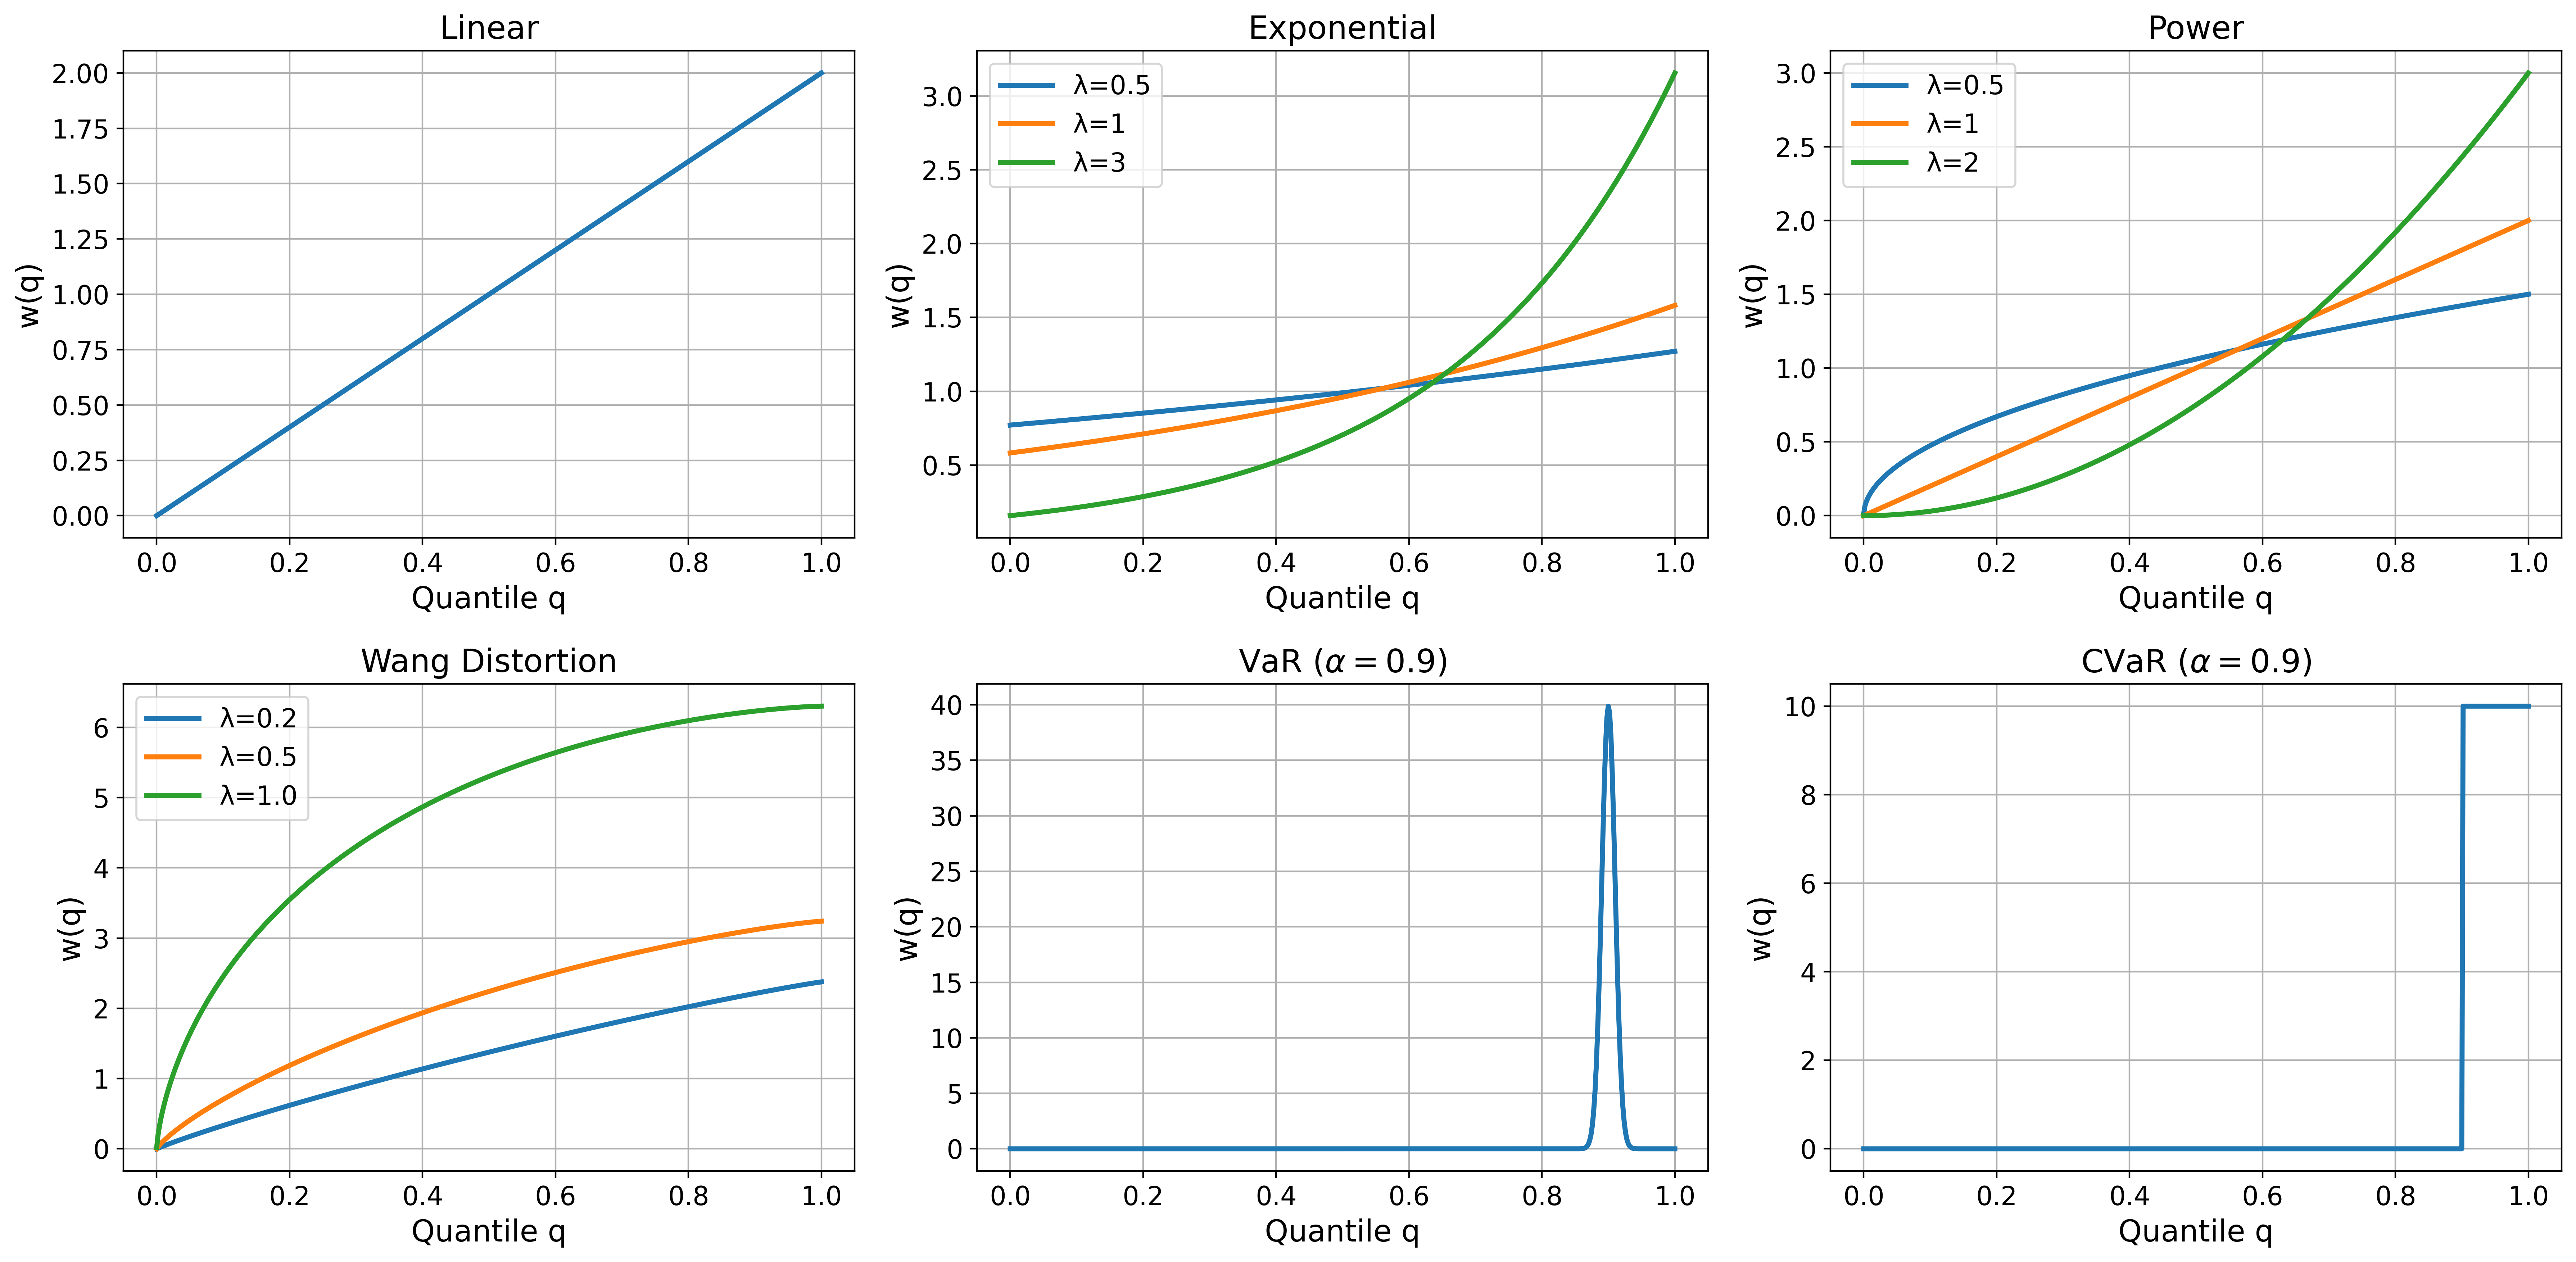
\includegraphics[width=0.9\textwidth]{figs/spectral_weights_comparison.png}
%     \caption{Illustration of spectral weighting functions corresponding to different spectral risk measures (SRMs). For parameterized families, the plots show how the spectral weights vary with the risk-aversion parameter $\lambda$.} \label{fig:srm-illustration}
% \end{figure}

% By selecting different quantile-weighting functions $w(q)$ in $\mathcal{L}_{\mathrm{FSD}}^w$, the FSD constraint can be tailored to enforce a variety of risk-sensitive behaviors. Uniform weights recover expected-cost minimization, extreme tail-focused weights recover Value-at-Risk or Conditional Value-at-Risk, and other schemes correspond to more general spectral risk measures. Thus, our framework provides a unified mechanism to impose different risk profiles simply by choosing $w(q)$, enabling principled, risk-aware alignment of policy behavior.
